% document based on the VU Beta / BSc Thesis template

\documentclass[11pt]{article}
\usepackage{graphicx}
\usepackage{hyperref}
\usepackage{booktabs}
\usepackage{listings}
\usepackage{multirow}
\usepackage[table,xcdraw]{xcolor}
\usepackage{appendix}
\usepackage{caption}
\usepackage{subcaption}
\colorlet{punct}{red!60!black}
\definecolor{background}{HTML}{EEEEEE}
\definecolor{delim}{RGB}{20,105,176}
\colorlet{numb}{magenta!60!black}

\lstdefinelanguage{json}{
    basicstyle=\tiny\ttfamily,
    numbersep=8pt,
    showstringspaces=false,
    breaklines=true,
    frame=lines,
    tabsize=2,
    backgroundcolor=\color{background},
    literate=
      {:}{{{\color{punct}{:}}}}{1}
      {,}{{{\color{punct}{,}}}}{1}
      {\{}{{{\color{delim}{\{}}}}{1}
      {\}}{{{\color{delim}{\}}}}}{1}
      {[}{{{\color{delim}{[}}}}{1}
      {]}{{{\color{delim}{]}}}}{1}
      {\ \ }{{\ }}{1}
}

      \textwidth 15cm
      \textheight 22cm
      \parindent 10pt
      \oddsidemargin 0.85cm
      \evensidemargin 0.37cm

%
\usepackage{xcolor}  % Colored text etc.
%
\definecolor{OwnAzure}{HTML}{336699}
\definecolor{OwnCerulean}{HTML}{CAE2FE}
\definecolor{OwnOliveGreen}{HTML}{556B2F}
%
\usepackage[colorinlistoftodos,prependcaption,textsize=tiny]{todonotes}% Add ,disable to the options, to hide the comments
%
%
\usepackage{xargs}                      % Use more than one optional parameter in a new commands
%
\newcommand{\todojacob}[1]{\todo[inline, color=OwnAzure!40]{Jacob: #1}}
\newcommand{\todoalexandru}[1]{\todo[inline, color=orange!40]{Alexandru: #1}}

\newcommand{\thoughts}[1]{\todo[inline, color=OwnOliveGreen!40]{Question: #1}}
\graphicspath{ {./images/} }
\begin{document}

\thispagestyle{empty}
\newcommand{\opendc}{OpenDC}

\begin{center}

Vrije Universiteit Amsterdam

\vspace{1mm}


\includegraphics[height=28mm]{vu-griffioen-white.pdf}

\includegraphics[height=28mm]{atLarge.jpg}

\vspace{1.5cm}

{\Large Bachelor Thesis}

\vspace*{1.5cm}

\rule{.9\linewidth}{.6pt}\\[0.4cm]
{\huge \bfseries LEGO, but with Servers:\par}
{\Large \bfseries Creating the Building Blocks to Design and Simulate Datacenters\par}\vspace{0.4cm}
\rule{.9\linewidth}{.6pt}\\[1.5cm]

\vspace*{2mm}

{\Large
\begin{tabular}{l}
{\bf Author:} ~~Jacob Burley ~~~~ (2599965)
\end{tabular}
}

\vspace*{1.5cm}

\begin{tabular}{ll}
{\it 1st supervisor:}   & ~~prof.dr.ir. Alexandru Iosup \\
{\it external collaborator:}   & ~~Georgios Andreadis \\
{\it 2nd reader:}       & ~~ir. Laurens Versluis

\end{tabular}

\vspace*{2cm}

\textit{A thesis submitted in fulfillment of the requirements for\\ the VU Bachelor of Science degree in Computer Science}

\vspace*{1cm}

\today\\[4cm] % Date

\end{center}

\newpage


\setcounter{tocdepth}{2}
\tableofcontents
\newpage
\listoffigures
\listoftables
\newpage


\section*{Abstract}
As consumption of cloud services grows, datacenters must increase in both number and capacity. 
Faced with a shortage of datacenter designers, it is important to make datacenter design accessible to a wider range of people, so that this growth may continue. 
In order to achieve this, we detail an extension to OpenDC that allows for the design of datacenters through the use of pre-designed building blocks, or \textit{prefabs}. 
We propose a hierarchical design for a data structure that allows for the representation of such building blocks.
Additionally, we design the accompanying methods that enable us to perform operations on prefabs. 
We design a prototype to test the suitability of our designs, allowing us to carry out an implementation of prefabs into the codebase of \opendc{}. 
We conclude that the addition of prefabs allows for a significant reduction in the number of interactions required (and thus the time taken) to build datacenters in \opendc{}. 
This result allows, not only for a faster means of iteratively improving datacenter designs, but also allows new users to get started with datacenter design much faster than they were previously able to.
\newpage

\begin{figure}
	\centering
	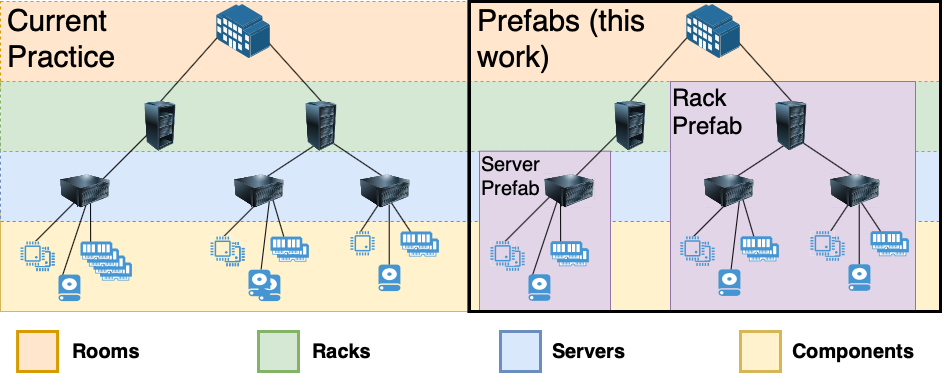
\includegraphics[width=\textwidth]{thesis_header.png}
	\caption[Prefabs in \opendc{} compared against the current approach of composing topologies]{Prefabs in \opendc{} compared against the current approach of composing topologies.}
	\label{fig:prefabsheader}
\end{figure}
\section{Introduction} \label{sec:introduction}
	With the rapid expansion in the use of cloud services by both consumers and businesses \cite{Kushida2015}\cite{mokhtar2013}, the datacenters that house these services must also grow. 
	While many consumers may not ever see the cloud in terms of its underlying hardware, cloud services are hosted on servers, and servers are typically stored in datacenters. 
	The configuration of such servers varies drastically, depending on the intended workload. 
	Relational databases, for example, can have large memory requirements\cite{Kabakus2017}. 
	Likewise, file servers may not need a particularly powerful CPU, but do require a lot of disks, and perhaps even a network card with higher maximum throughput\cite{Drapeau1994}.

	When architecting datacenters, many stakeholders must come together and agree on the various specifications of the data center, each with their own unique set of requirements. 
	System architects will then begin to design a system that meets these requirements. 
	However, such projects also have constraints. 
	Designing a data center is not as easy as buying servers that meet the requirements of the stakeholders and putting them into use. 
	Constraints such as budget or physical space often influence design decisions, with smaller (metropolitan) datacenters with less floor space sometimes making use of higher-density compute nodes, such as blade servers. 
	Designing datacenters is often a complex problem, for which no validated analytical models exist. 
	Despite some academic institutions often being forthcoming with the technologies used in their datacenters\cite{SURF2020}, there is no one-size-fits-all approach for data center design, making it hard to determine which hardware can support a given set of workloads.

	The shortage of up to 900,000 IT specialists by 2020\cite{Gareis2014} paired with the growing demand for datacenters, and thus datacenter architects, presents a significant problem.
	This raises the question: how can we continue to support such rapid growth in this sector, while the job market to support it does not grow to match?
	This research aims to extend existing datacenter simulation tools to allow them to be accessed by users with less of a technical background, enabling a broader audience of people to design datacenters.
	% As a result, we hope to further datacenter adoption by Small and Medium Enterprises, closing the existing gap between them and their Large Enterprise counterparts.

	\subsection{\opendc{}}
		Due to the financial, space and power requirements of server hardware, research into datacenter performance is more frequently being carried out with datacenter simulators.
		Such simulators provide the ability for researchers, and potential datacenter operators, to perform large-scale performance testing without having to make any capital expenditure in the process.
		In this way, prototyping becomes significantly cheaper, allowing for a much more flexible approach to datacenter research\cite{Iosup2017}.

		We focus in this work on \opendc{}, an open-source Discrete Event Simulator used to simulate the performance of workloads on massive computer systems\cite{Iosup2017}. 
		Its purpose is to assist in performance testing of datacenters designed by users, with the intention that the information gained can be factored in when these systems are being designed. 
		\opendc{} simulates workloads using traces from the Grid Workload Archive \cite{Iosup2008}, which are provided by participants who contribute to the archive, and are available to anyone through open-access. 
		These traces provide metadata about the scheduling requirements of jobs frequently sent to datacenters, such as CPU usage throughout a job. 
		Using this information in combination with information about the hardware being simulated, \opendc{} can simulate both the speed with which a workload will complete, and the resource usage throughout the workload. 
		These simulations can assist businesses and educational institutions in highlighting and addressing performance concerns in their next-generation environments before any hardware has even been purchased.

		Other simulators also exist, such as BIGSIM\cite{Zheng2004}, GridSim\cite{Buyya2002}, SimGrid\cite{Casanova2008}, and CloudSim\cite{Calheiros2011}.
		Among these datacenter simulators, \opendc{} claims to have the broadest range of performance-related features\cite{Andreadis2018}, and a comprehensive library of resource management techniques.
		As a result of these two characteristics, \opendc{} can express a wide range of possible datacenter scenarios.
	
	\subsection{Problem}
		In its current state, \opendc{} (and other simulators in the field) can be used to simulate user-specified workloads on user-designed systems. 
		In order to create these simulations, users must define a scenario in which the datacenter would be used, and specify each individual component used to build out an entire system, effectively doing all of the design work themselves. 
		This requires a high level of technical understanding, and relies solely on the user's knowledge of the intended workload to make component choices, as the user is responsible for choosing the hardware suited for that scenario. 
		
		Additionally, designing these datacenters is a time-consuming process, as there is no functionality to support the exporting or copying of existing designs.
		This means that even if a user has a defined scenario in which they want to use their datacenter and a design for that scenario, any reuse of components designed previously requires them to be completely recreated.
		Because the possibility of using a pre-existing design as a basis for a new design does not exist, non-technical users are faced with a steep learning curve when creating and experimenting with their own designs. 
		
		We envision that prefabricated components (\textit{prefabs}), that is, complete collections of components intended for a specific workload, could be ``dragged and dropped" into a datacenter design, allowing for accelerated prototyping.
		In this way, hardware choices could be made based on which workload(s) the user wants to run.
		As a result, all a user would need to know to begin designing a datacenter would be its intended purpose, the workloads it would be required to run, and some basic compositional rules for prefabs when trying to assemble more complex or advanced configurations.
		A visualization of this approach can be seen in Figure~\ref{fig:prefabsheader}.

		We also envision that users could export the topologies that they design as prefabs, allowing for easy replicability of existing designs.
		The ability to save their designs as prefabs could support the sharing of prefabs within communities, allowing others to benefit from the sharing of knowledge regarding hardware requirements for different workloads.
		Overall, we hope that the addition of such functionality would result in a collection of prefabs that covers a wide variety of workloads, across an even wider variety of hardware configurations.

		Additionally, prefabs could provide further benefits when working with scalable workloads.
		If the workload relies on homogeneous nodes, these nodes could be defined as prefabs, and added repeatedly into the design as needed for capacity testing.
		Prefabs could consist of a single server, but could also scale up to a rack full of servers, or even a room full of equipment.
		This approach would enable users reliant on homogeneous hardware configurations to save their standard configurations as prefabs, further saving time when they need to add more of the same kind of node in new designs.
	
	\subsection{Research Questions and Approach}
		In this thesis, we aim to improve the ease of use of \opendc{}, while also implementing a new, easily-expandable representation of datacenter hardware that allows for accurate technical descriptions of hardware. 
		In doing so, we answer the following three questions:
		\begin{itemize}
			\item [\textbf{RQ1:}] How to design a prefab abstraction that accurately describes important technical and composable features of datacenter hardware?

			It is important for our vision of prefabs to be able to store them in some way.
			In order to support this goal, we need to create a data structure that can contain an accurate hardware representation, along with its relevant metadata (such as tags, author, creation date etc).

			While smaller topologies may be expressed quite easily, we must consider that our solution should also scale to massive and complex topologies, while still preserving the same level of detail.
			It must also support a variety of operations to add, remove and modify data stored within it to facilitate users working with it.
			This data structure should also be relatively straight-forward to understand and easily extensible, allowing it to be further expanded by open source contributors.

			Our approach begins in Section~\ref{sec:design}, with understanding the shortcomings of the current implementation of topologies in \opendc{}.
			Next, we seek to understand the components that are important to represent in the data structure, and identify components we no longer need to represent.
			From here, we examine a variety of common methods of representing data, and assess their suitability towards our desired way of representing datacenter hardware.
			Following on from this, we present a data structure design, and the decisions made during the design process, validating our design by using it to represent servers currently offered by popular OEMs in Section~\ref{sec:evaluation}.
			We also assess what interactions need to be supported on the data structure, and ensure that the data structure design supports these interactions.

			% design section
			\item [\textbf{RQ2:}] How to implement a prototype of the prefab abstraction?
			% prototyping section

			Prototyping the prefab abstraction is important for the addition of prefabs, as we may use new technologies that need to be tested and evaluated for compatibility with the current \opendc{} software stack.
			We can use prototyping to become more familiar with these new technologies, analysing their strengths and potential shortcomings.
			We also may use prototyping to determine what is and is not useful in our initial data structure design, and iteratively improve our design with these findings.

			\opendc{} is quite a large and complex project, with a lot of moving parts.
			In the process of adding a new data structure throughout \opendc{}, it is important to continually test the code we are adding to the codebase for functionality.
			As a result, we must ensure that our prototype is representative of the structure of the current \opendc{} project.
			Then, we can add the functions and data structure to our prototype, and evaluate whether the interactions we have designed are suitable for further integration into the \opendc{} codebase.
			We can also use the prototype to determine if any additional changes need to be made to the existing codebase to support our extensions, and whether any of these modifications may adversely impact existing functionality.

			In Section~\ref{sec:prototype}, we detail the process of designing and creating a prototype.
			We also provide a summary of the lessons learned during prototyping, and describe how we can use what we have learned to further improve our implementation of prefabs into \opendc{}.
			% - mimicking the opendc project structure to create a basis, then defining methods of creating, modifying, fetching prefabs
			\item [\textbf{RQ3:}] How to assess the use of prefabs in practice?
			% KLM testing

			In addition to implementing prefabs, we also should show that they are important to the \opendc{} project, and to our goal of improving the usability of \opendc{}.
			To do this, we should assess the impact that the addition of prefabs has on performing certain tasks in \opendc{}, and determine what the benefits of prefabs are in concrete terms.

			In order to do so, we must devise a testing strategy to show the improvements that our prefab implementation brings.
			We must also decide which metrics are important to measure when showing these improvements, and how we can measure these quantities.

			In Section~\ref{sec:evaluation}, we detail our experimental setup for objectively testing the improvement that prefabs bring to \opendc{}.
			We also describe and discuss our experimental results, providing a short conclusion of what these results mean for the future of prefabs in \opendc{}.
			
		\end{itemize}
	
	\subsection{Main Contribution of the Work}
		This thesis pioneers a new approach to representing datacenter hardware within a datacenter simulator.
		The main contributions of this thesis are:
		\begin{enumerate}
			\item Envisioning the use of prefabs for the design and simulation of datacenters.
			\item The design of a data structure for storing datacenter hardware representations that is also easily usable and expandable, and an evaluation of said design in terms of the suitability of the data structure for purpose.
			\item An implementation of this design into the main codebase of \opendc{}, and an evaluation of this design comparing usability to the previous version of \opendc{}.
			\item An example library of components intended for High Performance Computing for use within \opendc{}, built using the design specified in this thesis.
		\end{enumerate}
	
	\subsection{Thesis Outline}
		The first section provides a short introduction to the current state of datacenter design, and the current state of OpenDC. 
		Section~\ref{sec:background} provides more background on how modularity is currently used in computing, both in datacenters and in fields such as software engineering. 
		In Sections~\ref{sec:design} and~\ref{sec:prototype}, we design a prefab data structure, reason about the choices that have been made during the design process, and touch on the process of implementing our chosen data structure into the \opendc{} codebase.
		Section~\ref{sec:evaluation} provides an assessment of the suitability of the data structure and technologies we chose, now that they have been implemented in \opendc{}.
		We assess both the implemented data structure, and the implemented methods of interacting with the data structure, using a different testing methodology for each.
		Finally, we discuss both the conclusion and future of this endeavour in Section~\ref{sec:conclusion}.
	

	

\newpage

\section{Background} \label{sec:background}
	Servers today are used for a wide variety of tasks, ranging from hosting video games all the way up to calculations for nuclear research at the European Organization for Nuclear Research (CERN) \cite{Andrade2012}.
	As the need for servers grows, in part due to a massive increase in the demand for cloud services \cite{Pring2009}, the size of datacenters will also have to grow.
	As a result, datacenter operators will have design and organise these new datacenters into a logical organisational structure.
	\subsection{Viewing Datacenters as Topologies}
		\begin{figure}[]
			\centering
			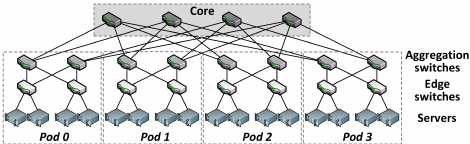
\includegraphics[width=\textwidth]{couto2012/Fat-tree-with-4-port-switches-n-4.png}
			\caption[A conventional network-focused datacenter topology]{A conventional network-focused datacenter topology \cite{Couto2012}.}
			\label{fig:networktopology}
		\end{figure}
		In general, individuals working with datacenters think about their datacenter in terms of its topology. 
		Often, this takes the form of a network topology \cite{Couto2012}, where a spanning tree is built from all of the participating nodes.
		An example of such a topology can be seen in Figure~\ref{fig:networktopology}. 
		For \opendc{}, however, it is also important to consider the positioning of hardware components within the topology.
		For example, we can consider a chassis residing within a given rack to be a child of that rack, with good datacenter practice requiring that an in-use chassis is not kept outside of a rack.
		By defining these inter-component relationships, we can build our own spanning tree model, which allows us to easily manipulate parent objects and all of their children by simply moving the parent object elsewhere in the tree, reshaping our topology.
		\begin{figure}[]
			\centering
			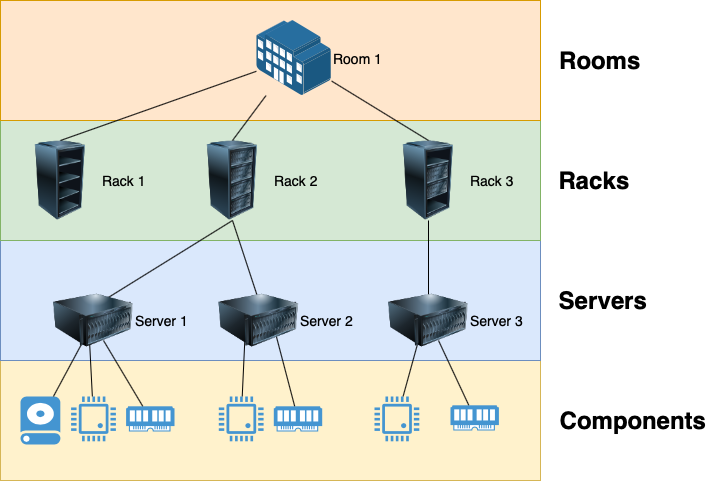
\includegraphics[width=8cm]{opendc-topology.png}
			\caption[A simple topology in OpenDC]{A simple topology in OpenDC.}
			\label{fig:example-opendc-topology}
		\end{figure}
	
	\subsection{Modularity in Computing}
		In software architecture, it is becoming increasingly common to rely on frameworks and libraries written by others in the software engineering community. 
		The programmer often only uses one or two functions from this library, and does not necessarily understand how these functions work (nor do they need to).
		It is usually not necessary to understand the full workings of such a library, as the benefit comes from its utility in meeting certain requirements. 
		We can view these software modules as prefabricated software, which an individual may add into their project with ease. 
		Such a module may be added manually, by copying the relevant source files into the project, or may be added by means of a package manager.
		
		\verb|npm| is a package manager for \verb|node.js| that seeks to make installing dependencies much easier for developers \cite{Wittern2016}.
		For open-source projects a developer can include a file listing all of the external packages they used in their project, and the specific versions of each of these packages, so that another individual can easily run the authors software on their own machine.
		\verb|npm| also enables package authors to publish their packages in an online registry, so that other developers may download and use them.
		It follows, then, that it would be helpful to be able to describe datacenter hardware, and share these descriptions, in a similar way. 

		With the emergence of \textit{Platform as a Service} (PaaS) and particularly \textit{Software as a Service} (SaaS) offerings from major cloud providers, developers can implement entire layers of their software stack with just a few clicks. 
		These layers still run in virtual machines, but the developer does not need to concern themselves too much with building or maintain the hardware or operating system.
		This concept is already offered by some cloud providers: DigitalOcean is a \textit{Virtual Private Server} (VPS) provider that harnesses a ``marketplace" of pre-configured VPS templates (known as ``1-Click Apps") to simplify use of the platform \cite{DigitalOcean2020}. 
		Customers can then easily add a pre-configured VPS to their environment, without having to worry about operating system installation, configuration, or maintenance. 
		Templates provided through the platform are typically created by the vendors of the software used in each template, and are thus of high quality and suitability for the chosen application.

		In the realm of hardware, we are also seeing modularity emerge. 
		Hewlett Packard Enterprise (HPE) produces a scalable server design, whereby more compute (in terms of CPU, Graphics and Memory) can simply be added as necessary \cite{Bang2020}.
		A single operating system instance runs on this hardware, which can (at the time of writing) be expanded with up to 4 nodes, each containing 32 sockets supporting up to 28 physical cores per socket.
		It is thus possible to begin with a single system, and simply add ``more of the same" when expanding datacenter capacity.

		At a more macro level, Schneider Electric provide prefabricated, modular structures to house, power, and cool datacenters \cite{Torell2014, Torell2017}.
		While the offering from Schneider Electric does not include recommendations for actual compute hardware, IBM offers the possibility of a completely modular datacenter \cite{IBM2014}.
		Such a datacenter can quickly be scaled up or down depending on the needs of the customer, using pre-designed components for power, cooling, and floorspace. 
		These prefab datacenters are real-life examples of how datacenter design can be modular.
	
	\subsection{Domain-Specific Modules}
		Datacenters have many intended uses, depending on the intended domain of the datacenter, such as High Performance Computing (HPC), scientific computing, business-critical applications, generalized cloud infrastructure, etc.
		The design of datacenters, and the component choices made during the design process, varies significantly depending on the domain it is used in.
		Some datacenter owners within the field of HPC may choose to focus on a hyperconverged infrastructure, where a many-core approach is taken to provide massive performance density.
		This allows for high performance, even within small metropolitan datacenters such as ones commonly found at universities, where space comes at a premium.

		In a business-critical environment, hardware may be physically replicated across both racks and physical locations, so that even a total datacenter loss would have a reduced impact on business operations.
		In such a scenario, hardware is not chosen based on the suitability for one application, but to support the flexibility to be able to run any application in virtual machines.
		This is especially common in this field, with the intention of further reducing downtime.
		Virtual machines can be migrated between physical hosts while still running when hardware maintenance is required.
		It is also possible to add resources to a virtual machine without power loss, dynamically scaling them to jobs.

		Conversely, other datacenter owners may focus on scientific computing \cite{SURF2020}.
		The requirements for such systems are different.
		They must support a high number of users, each with workloads that require as high a performance as possible.
		As a result, these datacenters are designed differently, with a high number of nodes running a baremetal operating system.
		The configuration of these nodes varies, depending on the intended use of the node.
		Nodes are then categorized into performance tiers based on their intended use.
		Performance tiers are then chosen by customers depending on the kind of workload they want to run - for example, GPUs may be installed in the nodes in tiers intended for Machine Learning workloads.

		Prefabs specific to certain domains can be represented in \opendc{}, with different performance tiers included within each domain.
		In this way, users can easily build massive, homogenous systems by selecting the node specific to their performance target, and using it as a starting point.

\newpage

\section{Designing Representation of Data Center Hardware} \label{sec:design}
	Servers within a datacenter are typically feature rich, with certain features included to differentiate them from their competitor.
	There are characteristics of the hardware (such as chassis colour) that have little relevance when designing a datacenter.
	Conversely, properties of the hardware such as the power draw, or the heat output, are important with regards to the planning of the datacenter infrastructure, as there will be a performance impact if these properties are not accounted for.
	When representing datacenter hardware in a data structure, it is important to consider which aspects of the hardware are relevant to represent.
	
	\subsection{Goal of Prefabs: Requirements Analysis}
		When designing our new data structure, it is important to consider the potential use-cases for key stakeholders.
		We identify our stakeholders to be researchers in the fields of distributed or large-scale computer systems, students in the same field, and datacenter operators in both industrial and academic settings.

		Both researchers and students would benefit from the addition of prefabs to \opendc{} in the same way that developers (and other customers) benefit from modern PaaS offerings, only having to focus on which services they want to run in their datacenter.
		Additionally, datacenter operators using \opendc{} for datacenter design and testing may also see a benefit from prefabs. 
		Cloud service providers who provide \textit{Infrastructure as a Service} (IaaS) services typically use homogenous hardware configurations, with different configurations for each performance tier. 
		With prefabs, it would be straightforward to create a prefab that is representative of a given performance tier, and then clone it when performing capacity planning during periods of growth.
		Lastly, given the widespread support for the sharing of information within academia, the ability to share prefabs would be an important addition to the features of \opendc{}.

		From these use-cases, we can already define some functional requirements for prefabs.
		\begin{itemize}
			\item [\textbf{FR1:}] Users should be able to use existing topology definitions as a basis for new prefabs.
			\item [\textbf{FR2:}] Users should be able to add prefabs into existing topologies, using them as building blocks to enable faster prototyping and design.
			\item [\textbf{FR3:}] Users should be able to determine what tasks a given prefab is suited for, by means of a labelling mechanism. Prefabs could then be labelled to indicate, for example, that they are intended for highly parallelizable workloads.
			\item [\textbf{FR4:}] Users should be able to easily share their prefab designs with others.
			\item [\textbf{FR5:}] \opendc{} should provide some example prefabs based on servers that are popular in the market. These prefabs would provide a building block for users to get started with.
		\end{itemize}

	\subsection{Model for Datacenter Representation}
		In this research, we provide a model for representing datacenter hardware, allowing us to store information  relevant to the simulation. Andreadis et al. created a similar model for datacenter hardware to model scheduling in \opendc{} \cite{Andreadis2018}, which serves as a basis for the model presented here. 
		When designing the model, we find it important to consider that a large part of its purpose is to increase the usability of \opendc{}. 
		As a result, we choose to represent hardware characteristics that are not used by the simulator, but provide useful information to the user. 
		Our model, therefore, offers more detail than the one presented by Andreadis et al, storing a wider range of the characteristics of the hardware components within.
		Hardware brands are not necessary to simulate workloads, but they are useful when a user is making design decisions, or presenting their design to a wider audience.
		Our model is broken down into different hardware components, each with different properties.
		These properties are detailed below.

		\subsubsection{Central Processing Unit(s)}
			A Central Processing Unit (CPU) in our model has four main characteristics: its name, its base clock speed in megahertz, the number of physical cores, and its energy consumption in Watts.
			With the exception of the name, all of these properties are important when performing a simulation of the performance of the CPU.
			A server is not limited in the number of CPUs it may contain.
			While commercially available servers, such as Lenovo's ThinkSystem SR950\footnote{\url{https://lenovopress.com/lp0647-thinksystem-sr950-server-xeon-sp-gen-1}}, may contain up to 8 CPUs in a single chassis, we choose not to place an artificial limit on the CPU count.
			In this way, the design of the data structure remains extensible, for both future hardware, and for entirely theoretical simulations.
			Additionally, this provides the flexibility required to represent multi-chassis servers, such as HPE's Superdome Flex\footnote{\url{http://hpe.com/superdome}}, that scale up to 32 sockets while functioning as one physical server to the operating system (and thus the workload).

		\subsubsection{Random Access Memory}
			In our model, Random Access Memory (RAM) has four primary characteristics.
			It has a human-readable name, a measure of its energy consumption in Watts, its capacity in megabytes, and its bandwidth in megabytes per second.
			The bandwidth of the memory is the product of its clock frequency, the number of data transfers per clock, the bus width of the memory, and the number of interfaces (modules) within the system.
			At the time of writing, server memory conventionally uses Double Data Rate (DDR), with a 64-bit bus width.
			The bandwidth of each module is calculated as if it were the only module in the system.
			The combined memory bandwidth of a system therefore increases linearly as we add modules.
			We choose again not to limit the number of memory modules that can be added to a system.
			While our findings suggest that Lenovo's aforementioned ThinkSystem SR950 has the most memory modules of any single-node system, with 96 in total, we do not want to artificially constrain researchers and datacenter operators from experimenting with theoretical systems with much higher memory density.

		\subsubsection{Graphics Processing Unit(s)}
			When representing Graphics Processing Units (GPUs), we represent its name, the number of GPU cores it contains, the clock speed of the GPU cores, and the power consumption.
			For the purposes of supporting theoretical hardware definitions, there is no limit on the number of GPUs that can be added to a topology. 
			This choice additionally supports the simulation of systems that use an external chassis to house GPUs, using PCI Express to connect to the main compute chassis, such as the One Stop Systems 3U Compute Accelerator\footnote{\url{https://www.onestopsystems.com/3u-compute-accelerator-nvidia-tesla-gpus}}, which supports up to 16 GPUs per external chassis. 

		\subsubsection{Storage}
			In our storage representation, we model the properties currently required for storage simulation within \opendc{}.
			These include the name of the device, its size in megabytes, its peak read speed in megabytes per second, and its peak power usage in watts.
			There is no limit on the number of drives that a system can include, in order to support theoretical hardware definitions.
			Additionally, this lack of limit allows for the simulation of systems that may rely on external disk arrays (such as NetApp's DS460C\footnote{\url{https://www.netapp.com/us/products/storage-systems/disk-shelves-and-storage-media/index.aspx}}) for storage, as \opendc{} currently does not include support for storage topologies such as \textit{Storage Area Networks} (SANs).
	
	\subsection{Definition and Design of a Data Structure for Storing Prefabs}
		In order to store our datacenter hardware representation within \opendc{}, we define a new data structure.
		When considering a new format for representing our data structure, we must first identify a suitable format that meets the requirements necessary for this project: to be human-readable and compatible with the existing \opendc{} software stack.

		The database used in version 1.x of \opendc{} contains 35 SQL tables, 20 of which are used to store topologies.
		As a result, adding hardware items to the database requires a complex set of queries, with deletions and modifications requiring additional queries.
		In order to reduce the complexity associated with \opendc{}, we seek a storage format that allows us to store entire prefabs (and topologies) within a single object.
		The advantage of such an approach is that the database then supports the adding, updating and deleting of prefabs and other topology objects, without the use of complex queries.
		We therefore consider several new formats for representing our data structure.

		First, we consider \textit{YAML Ain't Markup Language} (YAML)\footnote{\url{https://yaml.org/spec/1.2/spec.html}} as our document format.
		YAML supports nested object hierarchies, however we argue that YAML is not suitably human-readable.
		It relies on indentation for distinguishing levels of hierarchy, with no clear boundaries delimiting separate objects.

		\textit{Extensible Markup Language} (XML)\footnote{\url{http://www.w3.org/TR/REC-xml}} is a common language for storing and representing documents that is used in many web applications.
		It is both human and machine readable by design, and is well suited to nested object hierarchies, making it a strong contender to be used to store prefabs.
		However, XML requires parsing.
		The current \opendc{} frontend is written in \verb|ReactJS|, which does not natively support parsing XML without the use of an external library.
		As we prefer not to add additional dependencies to \opendc{}, we do not find XML to be a suitable choice as a document format.

		Lastly, we consider \textit{JavaScript Object notation} (JSON)\footnote{\url{https://www.json.org/json-en.html}}.
		JSON is an expressive, industry-standard object storage format that is widely used in web-based applications.
		It is both human-readable, and supports nested object hierarchies.
		The support for nested objects is crucial to us to achieve some of our functional requirements, namely \textbf{FR1} and \textbf{FR2}, as it allows for easier insertion into the object.
		In addition, it is supported by the standard libraries available in both Python and ReactJS, making it ideal for our data structure storage format.
		As a result, we choose JSON as a means to store our prefab data structure.
		
		This JSON-based data structure aims to be simple to understand, and easily expandable to represent hardware configurations that we do not focus on in this research (i.e. blade servers, or other chassis that may contain multiple/unconventional motherboards).
		This means that, along with the default fields for components we have previously specified, it is easy to add new fields to components in the future by simply adding new fields to the object.


	\subsection{Designing Ways to Create and Interact with Prefabs}
		When determining interactions with prefabs, we must define a set of operations that meets the functional requirements previously defined.
		
		From \textbf{FR1}, we can make the case for functionality that would allow a prefab to be created from an existing topology.
		Such functionality should create a copy of the current topology, and store it as a prefab, allowing the user to determine the visibility (private or public) and name of the prefab.

		The ability to save topologies as prefabs also serves as the basis for the behaviour highlighted in \textbf{FR2}, where users would be able to then create new topologies from prefabs, or add prefabs into their existing topologies.
		Users would be able to choose from their own private prefabs, and from all public prefabs, when adding prefabs into their design.

		Users would also be able to find prefabs based on their intended use, amongst other labels. 
		Such behaviour would be made possible by means of a labelling mechanism, satisfying \textbf{FR3}.
		This labelling mechanism would take the form of an additional field on the prefab object, storing an array of tags assigned to the prefab.
		These tags would indicate the suitability of the prefab to a specific task, but could also be used to indicate the scale at which it can execute such a task.
		Such labellings are already used to convey the size of IaaS instances offered by cloud providers \cite{davatz2017}, and could also be used by \opendc{} to convey the size of workload a prefab is designed to execute.

		The aforementioned labelling mechanism, combined with the ability to mark a prefab as public or private, would be crucial to enable the sharing of prefabs between users mentioned in \textbf{FR2}.
		Such a sharing mechanism should allow users to search for prefabs, or filter them based on common tags.
		This would enable users to find prefabs created for specific tasks, and easily share prefabs for new tasks with the community, as highlighted in \textbf{FR4}.

		Lastly, the inclusion of some \opendc{} prefabs outlined in \textbf{FR5} is important to provide a basis for new prefabs.
		Such a provision would also provide a reference for how prefabs can look to users unfamiliar with them.
		It would also provide the means to immediately get started with creating topologies from prefabs, instead of waiting for the community to begin providing their own.
		Additionally, the inclusion of some basic prefabs in \opendc{} would allow users to benefit from prefabs even if they are self-hosting \opendc{}, without the community contributions.

\newpage

\begin{figure}[]
	\centering
	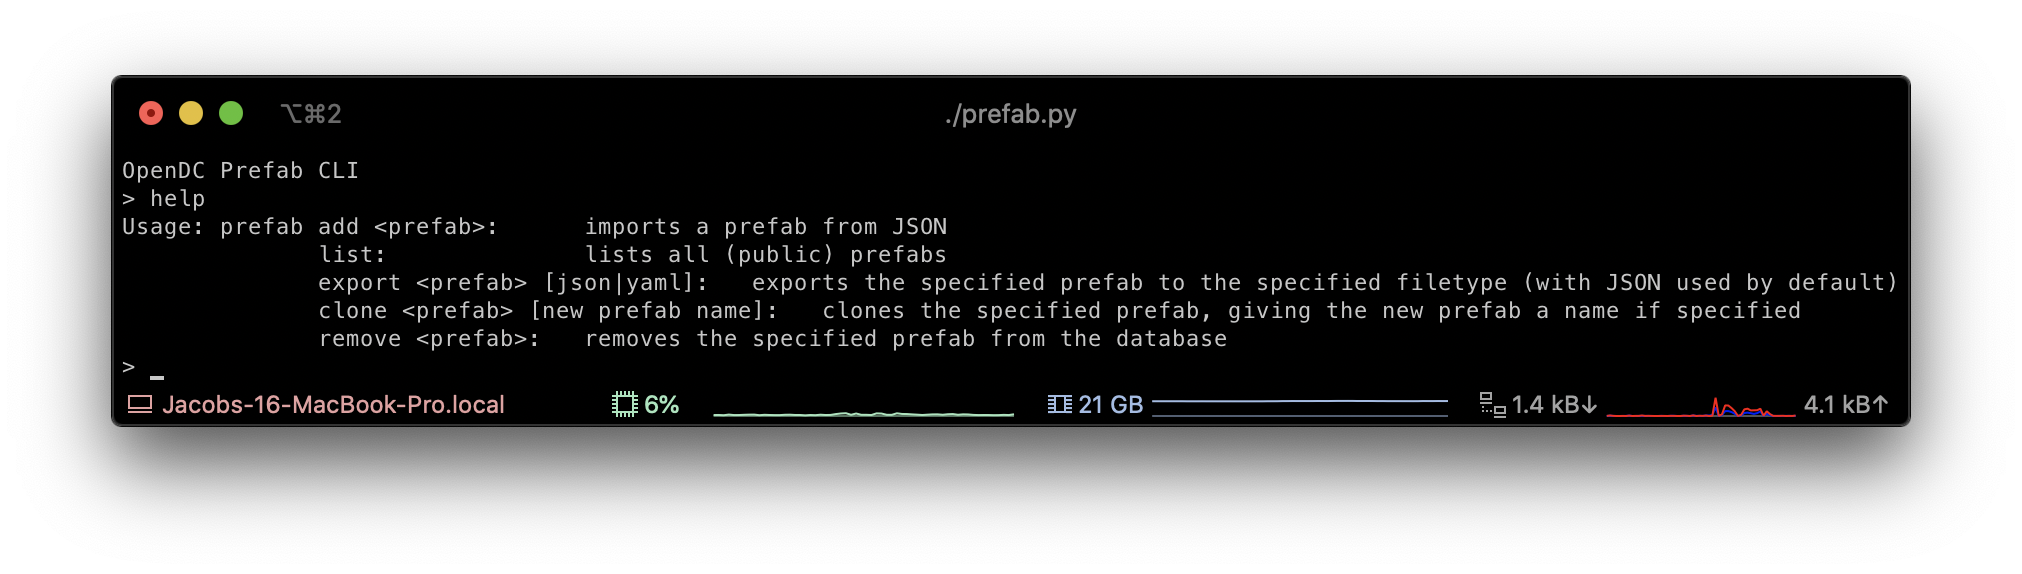
\includegraphics[width=\textwidth]{prototype1.png}
	\caption[Prototype showing the CLI operations it supports]{Prototype showing the CLI operations it supports.}
	\label{fig:prototype1}
\end{figure}
\begin{figure}[]
	\centering
	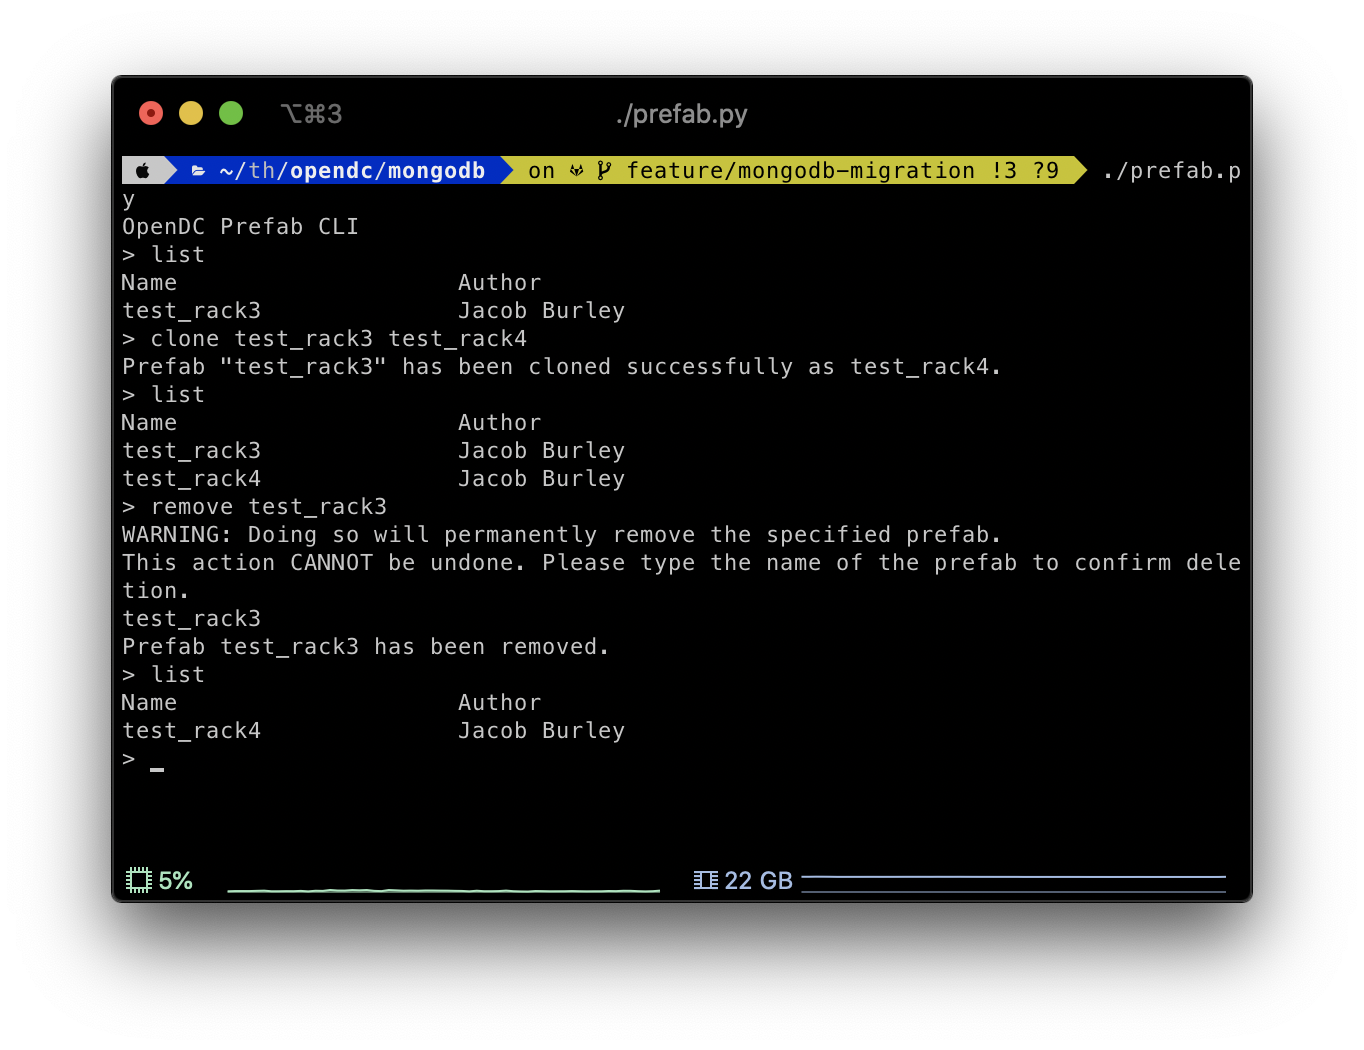
\includegraphics[width=0.8\textwidth]{prototype2.png}
	\caption[Prototype demonstrating the import and deletion of a topology module]{Prototype demonstrating the import and deletion of a topology module.}
	\label{fig:prototype2}
\end{figure}


\section{Implementation of a Prototype} \label{sec:prototype}
	In this section, we describe the prototyping stage of this project.
	We cover the motivations behind prototyping, and the processes of designing, implementing and testing the prototype.
	\subsection{Why Prototype?}
		Prototyping is an important part of our design process for implementing the new topologies in \opendc{}.
		In order to further the goal of simplifying working with \opendc{}, we have chosen to transition the storage database away from SQL, towards a NoSQL design.\footnote{The author of this thesis was involved in the transition from SQL to NoSQL, involving the implementation of the new databse, and the porting of the current database schema to MongoDB. 
		This effort also involved porting the existing \opendc{} API from Python 2.7 to Python 3, and rewriting the API to include new endpoints for prefabs, and the new topology structure.}
		MongoDB has been chosen by the \opendc{} team as a NoSQL document storage solution due to its ease of use, and its flexibility.
		MongoDB additionally natively supports the insertion of JavaScript Object Notation (JSON) objects, which we use as the storage format for our data structure.
		It also provides strong library support for Python via the \verb|pymongo| module, supporting the integration of the new database structure with the \opendc{} API.

		As a result, prototyping provides us with a way of becoming familiar with these new technologies, and assessing their suitability, before we begin the process of implementing them into the existing \opendc{} codebase.
		Prototypes of the data structure and its interactions are also important to assess the whether the data structure 
		We also can create prototypes of the data structure, and the corresponding interactions with it, and assess the suitability of the data structure with regards to the interactions we require it to perform.

		In addition to the above reasoning, we also consider that \opendc{} uses a combination of ten different technologies to provide its service.
		In the frontend, JavaScript, React, Redux, and Konva are used. For the webserver and API, \opendc{} uses Python, Flask, FlaskSocketIO, and OpenAPI.
		MariaDB is currently used as the database for storing topologies, simulations and experiments, and the simulator itself is written in Kotlin.
		Due to the significant change to the software stack that a transition to MongoDB represents, we must use our prototype to test the compatibility of our design in the existing context of \opendc{} to make sure that our design (and MongoDB) is a viable addition to \opendc{}.

	
	\subsection{Creating a Prototype}
		The two main goals of prototyping are to explore how we can best implement and interact with MongoDB, and to iteratively improve our data structure design.
		As a result, the prototype consists of three components: a MongoDB instance, a Python module that interfaces with the database, and a second Python application to serve as a rudimentary frontend. 
		This configuration has been chosen to be relatively close to how \opendc{} already implements its database connections, which also uses a Python module to abstract away most database interactions.

		MongoDB has been chosen as a database replacement, as it easily facilitates the storage of our JSON objects.
		MongoDB stores documents in a JSON-like format internally, and has strong library support for inserting, modifying and exporting said documents, making it relatively straightforward to re-implement our database connection.

		Because we are able to insert nested JSON objects into MongoDB, we do not need to rely on multiple tables and foreign keys used in a typical relational database like MariaDB.
		We can simply store the entirety of a topology in a single document within MongoDB, and access specific fields within those documents when we need to.
		As a result, our implementation of MongoDB relies on simpler queries than SQL, as we can simply get the object into memory, modify it, and re-insert it into the database with two queries.
		We do not have to update each table and foreign key when we modify a prefab.

		The resulting prototype frontend takes the form of a command-line interface for interacting with prefab objects (shown in Figure~\ref{fig:prototype1}).
		This prototype is capable of performing some basic operations on prefabs, such as importing a prefab from a JSON file on the local filesystem and adding it to the database, exporting a prefab to a JSON file on the filesystem, cloning a prefab, listing all prefabs available in the database, and deleting prefabs.
		Such behaviour can be seen in Figure~\ref{fig:prototype2}.
		The functionality modelled covers the most essential functions that a prefab implementation requires, with the listing functionality even including some rudimentary access control support.
		It also serves as a useful test of the functionality of MongoDB, and provides sufficient reference material for the implmentation of a MongoDB connection in the API of \opendc{}.

	\subsection{Lessons Learned}
		During prototyping, we learnt many things that influenced the decisions we made during the implementation phase.

		Firstly, we opted not to enforce schema validation on the collections within our database.
		The reasoning behind this decision was that schema validation in the database added unnecessary complexity, and limited the shape of our data (and thus hardware that could be represented).
		We instead choose to check for required fields (such as the topology name, or the prefab visibility) within the API.
		This allows for topologies to contain hardware configurations that may not have been considered during the design process, while also allowing us to make assumptions about certain aspects of the data structure.

		We also became more familiar with certain aspects of MongoDB, including the differences between Binary JSON (BSON) and JSON.
		When we began working with MongoDB, we operated under the assumption that MongoDB would export objects in JSON, just as it can be given JSON objects to import.
		However, this assumption turned out to be incorrect. 
		During testing of topology import functionality, we attempted to import a topology that we had exported to JSON.
		When this test failed, we discovered that MongoDB does not use pure JSON for exports.
		Instead, it exports objects in BSON, the same format it uses to store objects internally within the database.
		MongoDB simply stores files in a binary format internally, and converts them back to something human-readable when you export them. 
		However, the human-readable format that MongoDB uses is not JSON, but is deceptively similar: BSON uses single quotes (\verb|'|) where JSON uses double quotes(\verb|"|).
		As a result, we implemented a conversion from BSON to JSON within our API, so API responses are formatted in proper JSON that can be used by the frontend.
		


\newpage

\begin{table}[]
\centering
	\begin{tabular}{lr}
	\toprule
	Operator                                              & Time taken (seconds) \\ \midrule
	K (keystroke or button press)                         & .75                  \\
	P (point to a target on a display with a mouse)       & 1.1                  \\
	H (homing hands on keyboard or other device)          & 0.4                  \\
	M (mentally preparing for executing physical actions) & 1.35                 \\
	B (mouse button press or release)                     & 0.1                  \\
	R (system response time)							  &	   0.1                  \\
	\bottomrule
	\end{tabular}
\caption[Relevant KLM operators used in our testing, and their times to complete]{Relevant KLM operators used in our testing, and their times to complete\cite{Newell1980}.}
\label{tab:3}
\end{table}


\begin{figure}[]
	\centering
	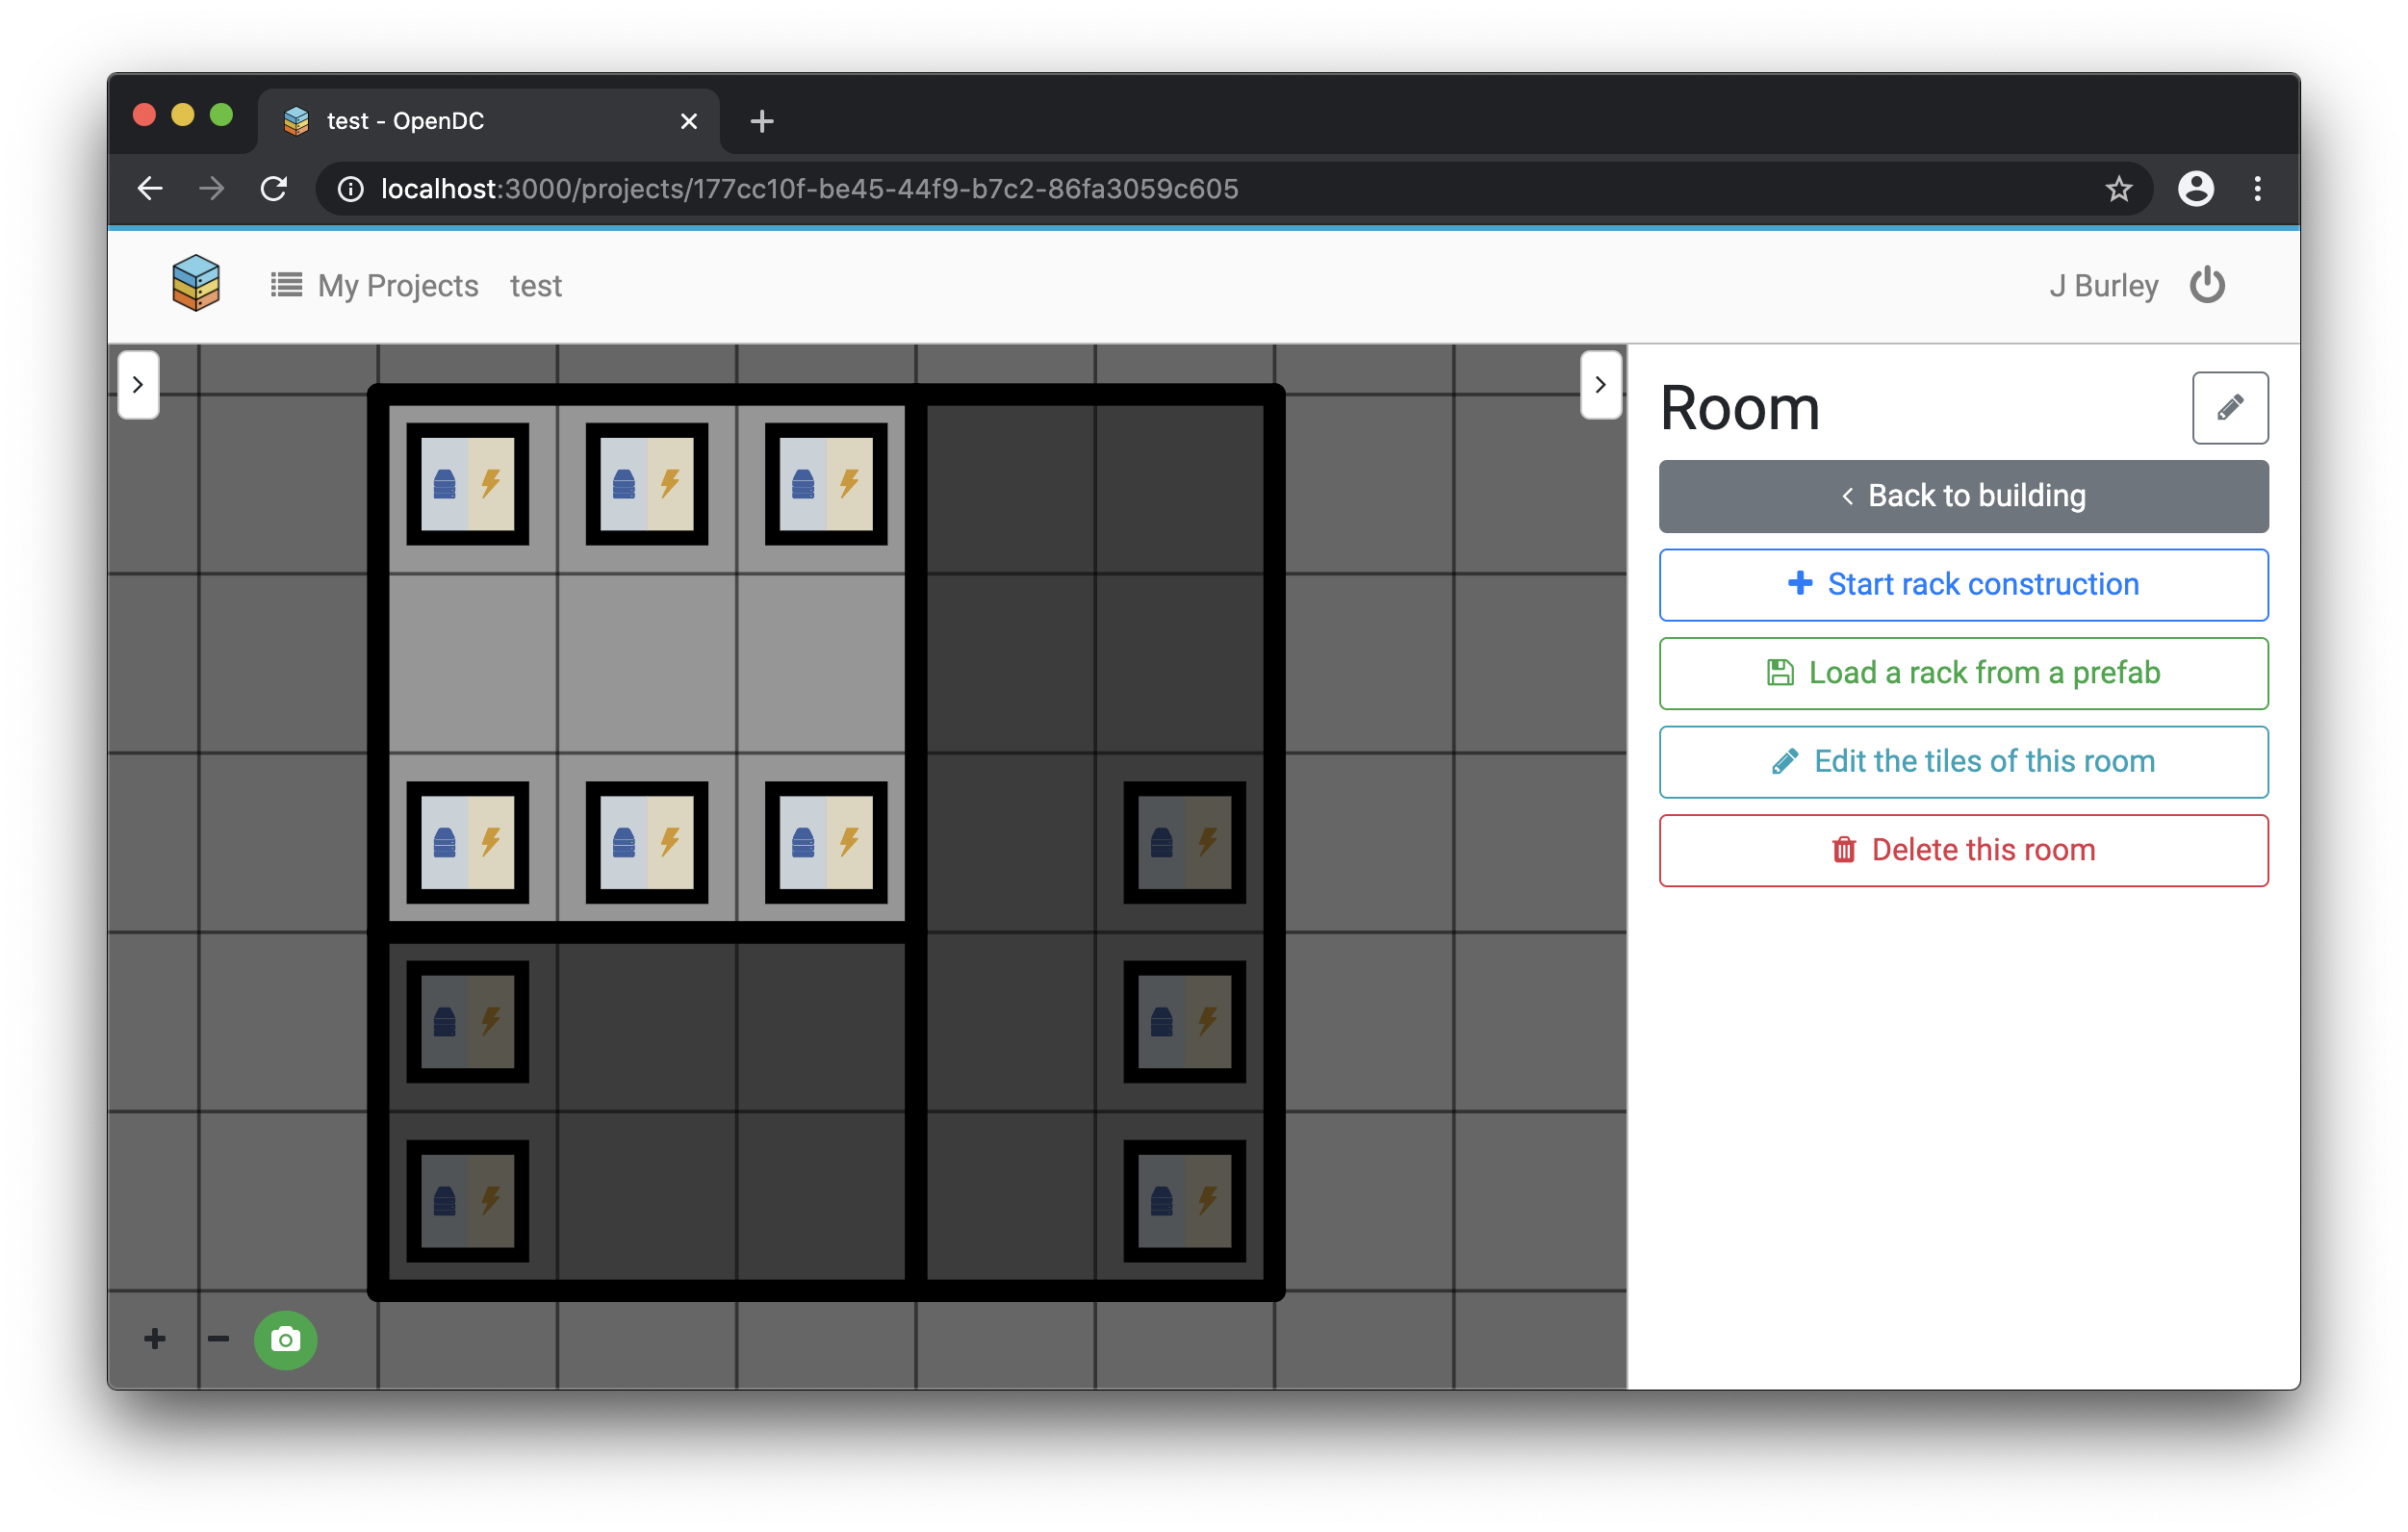
\includegraphics[width=\textwidth]{frontendstartingpoint.png}
	\caption[The starting position for evaluation]{The starting position for evaluation. Screenshot taken from OpenDC extended with our work.}
	\label{fig:evalstart}
\end{figure}

\section{Evaluation of Design \& Implementation} \label{sec:evaluation}
	In this section, we evaluate the success of both the design, and the implementation of our prefab data structure.
	We do this in two ways: first, we test the ability of prefabs to represent real-life hardware, as per \textbf{RQ1}.
	Secondly, we use a popular Human Computer Interaction model to assess the success of the implmented operations on prefabs, as per \textbf{RQ3}.

	\subsection{Evaluating the Design with Domain-Specific Prefabs}
		In this section, we explore the High Performance Computing domain, and validate our prefab representation by creating prefabs for some of the HPC-oriented server offerings from the top 3 OEMs by market share in Q1 2020.
	
		\subsubsection{Representing Domain-Specific Hardware with Prefabs}
			\begin{table}[]
			\centering
				\begin{tabular}{lrr}
				\toprule
				Company                     & Units Shipped      & Market Share     \\ \midrule
				\rowcolor[HTML]{9AFF99} 
				Dell Technologies           & 474,011            & 18.4\%           \\
				\rowcolor[HTML]{9AFF99} 
				HPE/New H3C Group           & 377,544            & 14.7\%           \\
				\rowcolor[HTML]{9AFF99} 
				Inspur/Inspur Power Systems & 211,007            & 8.2\%            \\
				Lenovo                      & 153,570            & 6.0\%            \\
				Super Micro                 & 132,001            & 5.1\%            \\
				ODM Direct                  & 770,446            & 29.9\%           \\
				Rest of Market              & 456,841            & 17.7\%           \\ \midrule
				\textbf{Total}              & \textbf{2,575,439} & \textbf{100.0\%} \\ \bottomrule
				\end{tabular}
			\caption{Market share distribution amongst server OEMs in Q1 of 2020.}
			\label{tab:1}
			\end{table}
			\begin{table}[]
			\centering
				\begin{tabular}{llrrrr}
					\toprule
					Brand       & SKU        & CPUs & DIMMs & Drives & GPUs \\ \midrule
					Dell                 & PowerEdge R440      & 2             & 16             & 10              & 0             \\
					Dell                 & PowerEdge R640      & 2             & 24             & 10              & 0             \\
					Dell                 & PowerEdge R740xd    & 2             & 24             & 24              & 0             \\
					Dell                 & PowerEdge R940      & 4             & 48             & 24              & 0             \\
					HPE                  & Superdome Flex Node & 4             & 48             & 4               & 4             \\
					HPE                  & DL360 gen10         & 2             & 24             & 8               & 0             \\
					HPE                  & DL380 gen10         & 2             & 24             & 24              & 0             \\
					HPE                  & DL580 gen10         & 4             & 48             & 48              & 0             \\
					Inspur               & NF5280M5            & 2             & 24             & 25              & 0             \\
					Inspur Power Systems & FB5180G2            & 2             & 16             & 10              & 0             \\ \bottomrule
				\end{tabular}
			\caption{Overview of the HPC prefabs created for this thesis.}
			\label{tab:2}
			\end{table}
			\newpage
			\begin{figure}[]
			\centering
				\begin{lstlisting}[language=json]
{
	"_id" : 440,
	"name" : "Dell R440",
	"tags" : ["hpc"],
	"visibility" : "public",
	"rack" : {
		"name": "Dell R440",
		"capacity": "42",
		"powerCapacityW": "25000",
		"machines" : [
			{
				"position": 1,
				"cpus": [
					{
						"name": "Intel Xeon Gold 6252",
						"clockRateMhz": 2100,
						"numberOfCores": 24,
						"energyConsumptionW": 150
					},
					...
				],
				"gpus": [],
				"memories": [
					{
						"name": "SK Hynix RDIMM HMA84GR7MFR4N-VK",
						"speedMbPerS": 42656,
						"sizeMb": 32768,
						"energyConsumptionW": 10
					},
					...
				],
				"storages": [
					{
						"name": "Dell 1.92TB SSD SATA",
						"speedMbPerS": 600,
						"sizeMb": 1920000,
						"energyConsumptionW": 10
					},
					...
				],
			}
		]
	}
}			\end{lstlisting}
				\caption[An example of a topology module for a Dell PowerEdge R440]{An example of a prefab for a Dell PowerEdge R440.}
				\label{fig:3}
			\end{figure}

			In order to select server SKUs to represent, we identify the top server OEMs by market share in Q1 of 2020 \cite{Macatee2020}. These summarised findings are presented in Table~\ref{tab:1}.
			We choose the three individual manufacturers with the largest market shares (highlighted in green) as our target manufacturers.
			We then choose the HPC-oriented server offerings from each of these manufacturers, and attempt to model them in the prefab data structure.
			
			The server selection process varies slightly by manufacturer, but generally, we seek out servers that the manufacturer describes to be suited for HPC, or other intensive compute workloads.
			For each server, we then attempt to represent it with as powerful of a configuration as possible, populating all sockets, DIMM slots and storage bays.
			For HPE's Superdome Flex, we also include the optional GPUs in the configuration.
			Other configurations present support GPUs, but as they are not included in any of the available OEM configurations, we opt not to include them in these configurations.
			Additionally, we choose not to include hardware from New H3C Group, as these servers are rebranded variants of the hardware already produced by HPE.
			As a result, the configurable options remain exactly the same as those of their HPE counterparts.

			The variety of hardware configurations in the resulting prefabs is shown in Table~\ref{tab:2}.



		\subsubsection{Accuracy of Hardware Representation}
			Ultimately, we argue that the accuracy of our hardware representations (a condensed example of which is given in Figure~\ref{fig:3}) is sufficient.
			The characteristics of the chosen hardware representable in our data structure are sufficient for simulation of that hardware in \opendc{}, so the prefabs created are functional in terms of being able to use them as part of a topology to be simulated.
			However, there are aspects of each server that are not represented in our prefabs, such as the presence of Out-of-Band management, or network cards.
			These components currently do not form part of our topology design, as they are currently not relevant to our simulations.

			Additionally, there are aspects of hardware that we have chosen not to represent in this thesis, such as multi-node chassis.
			As a result, it was not possible to model hardware such as HPE's ``Apollo" line of high-density HPC servers\footnote{\url{https://www.hpe.com/us/en/storage/apollo-4000.html}}, or Dell's PowerEdge Blade Enclosure\footnote{\url{https://www.dell.com/ly/business/p/poweredge-m1000e/pd}}.
			Such hardware is seen frequently in the HPC domain, providing high levels of compute density, further solidifying the notion that \opendc{} should support these kinds of representations in the future.
			However, it is still possible to simulate performance aspects of these multi-node systems, as they can be represented within \opendc{} as individual servers.
			As a result, this limitation only impacts physical datacenter design.

			Lastly, the ``Inspur Power Systems FP5180G2" prefab contains IBM POWER9 processors, based on the Power Instruction Set Architecture \cite{IBM2017}.
			These CPUs exhibit different performance characteristics than Intel or AMD processors, in part due to different instructions exposed by the CPU.
			This difference is not accounted for by the simulator in \opendc{}, and there is currently not a provision for representing this difference in our topology structure.
			Again, this is an improvement that could be made in the future, and would be relatively straightforward to represent given the flexible nature of our topology structure.


		\subsubsection{Applying the Prefabs Approach to Other Domains}
			We argue that this approach would be straightforward to apply to other domains.
			Most manufacturers split their hardware offerings up according to their intended workloads, allowing for relatively straightforward server selection.
			For smaller domains (such as game streaming), however, it may be beneficial to consider the performance requirements of the domain with regards to specialized hardware, as these domains are not always as clearly differentiated.

	\subsection{Evaluating the Use of Prefabs in Practice}
		In this section, we evaluate the performance improvements resulting from the implementation of prefabs.
		We use the \textit{Keystroke-Level Model} (KLM) \cite{Newell1980} to test the duration of performing a given task in both versions of \opendc{}, and compare the results.
		KLM measures the number of keystrokes (or other actions) that need to be executed to complete a given goal. 
		Each action is assigned a time duration.
		In order to calculate an estimate of how long a task will take, one can map out the actions required to complete the task and translate these actions directly to a time duration.

		\subsubsection{Experimental Setup}
			When evaluating our implementation, we must compare our additions to \opendc{} to a version of \opendc{} before our extensions were added.
			For the purposes of our comparison, we will use the aforementioned KLM methodology to test the duration of executing a specific task.
			We present a subset of the KLM operators in Table~\ref{tab:1}.

			As part of our testing, we account for the response time of the system. 
			While we observed that, once the application is loaded locally, it reacts quite quickly (almost instantly) to user interaction.
			However, in this scenario the application is running on a local machine, with only one user.
			In a production environment we would expect both multiple concurrent socket connections due to multiple users, and increased latency between the server and the client when they are not on the same host. 
			As a result, we use an \textit{R} value of 0.1 seconds to represent the time the system takes to update the user interface, as we feel this is more representative of how the system would behave when deployed.
			This value will be added to our final total for each click of the mouse (\textit{B}).
			We also make the assumption that the user has their hand on the mouse already, negating the need to include the duration required to home their hand to the mouse.

			For our usability test, we compare the process of copying a rack in version 1.x of \opendc{}, and our new version of \opendc{} with prefabs.
			We create a room, containing a single rack.
			This rack contains 3 machines, each containing 1 CPU, 1 GPU, 1 memory DIMM, and one hard disk.
			We then attempt to copy the contents of this rack into a new rack.
			The KLM task begins on the screen shown in Figure~\ref{fig:evalstart}, and ends when a second rack has been created with the same contents as the initial rack.
			

		\subsubsection{Experimental Results}
			\begin{figure}
				\centering	
				\begin{subfigure}[b]{\textwidth}
					\centering
					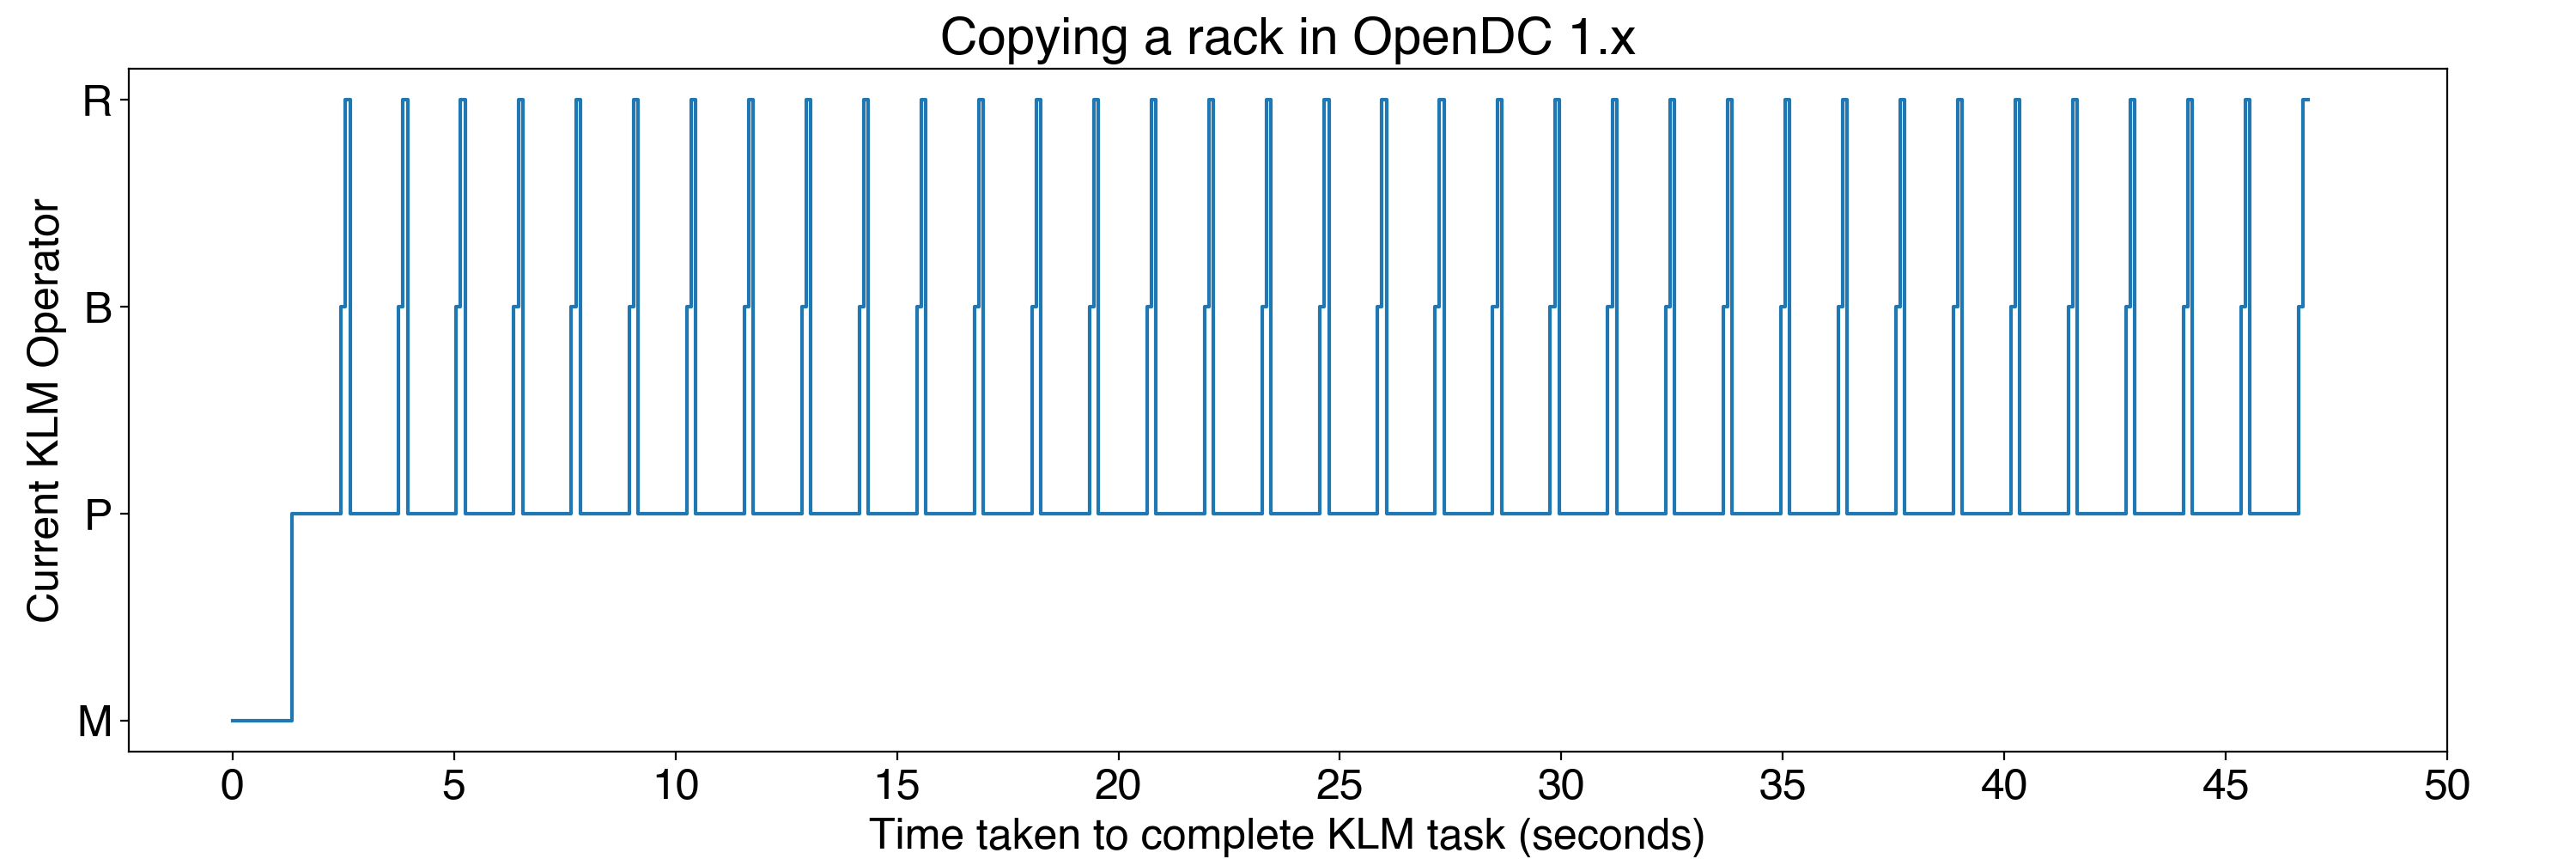
\includegraphics[width=\textwidth]{results/opendc1.png}
					\caption[Graph showing interactions required to complete a KLM task in \opendc{} without our extensions]{Graph showing interactions required to complete a KLM task in \opendc{} without prefabs.}
					\label{fig:opendcklm1}
				\end{subfigure}
				\vfill
				\begin{subfigure}[b]{\textwidth}
					\centering
					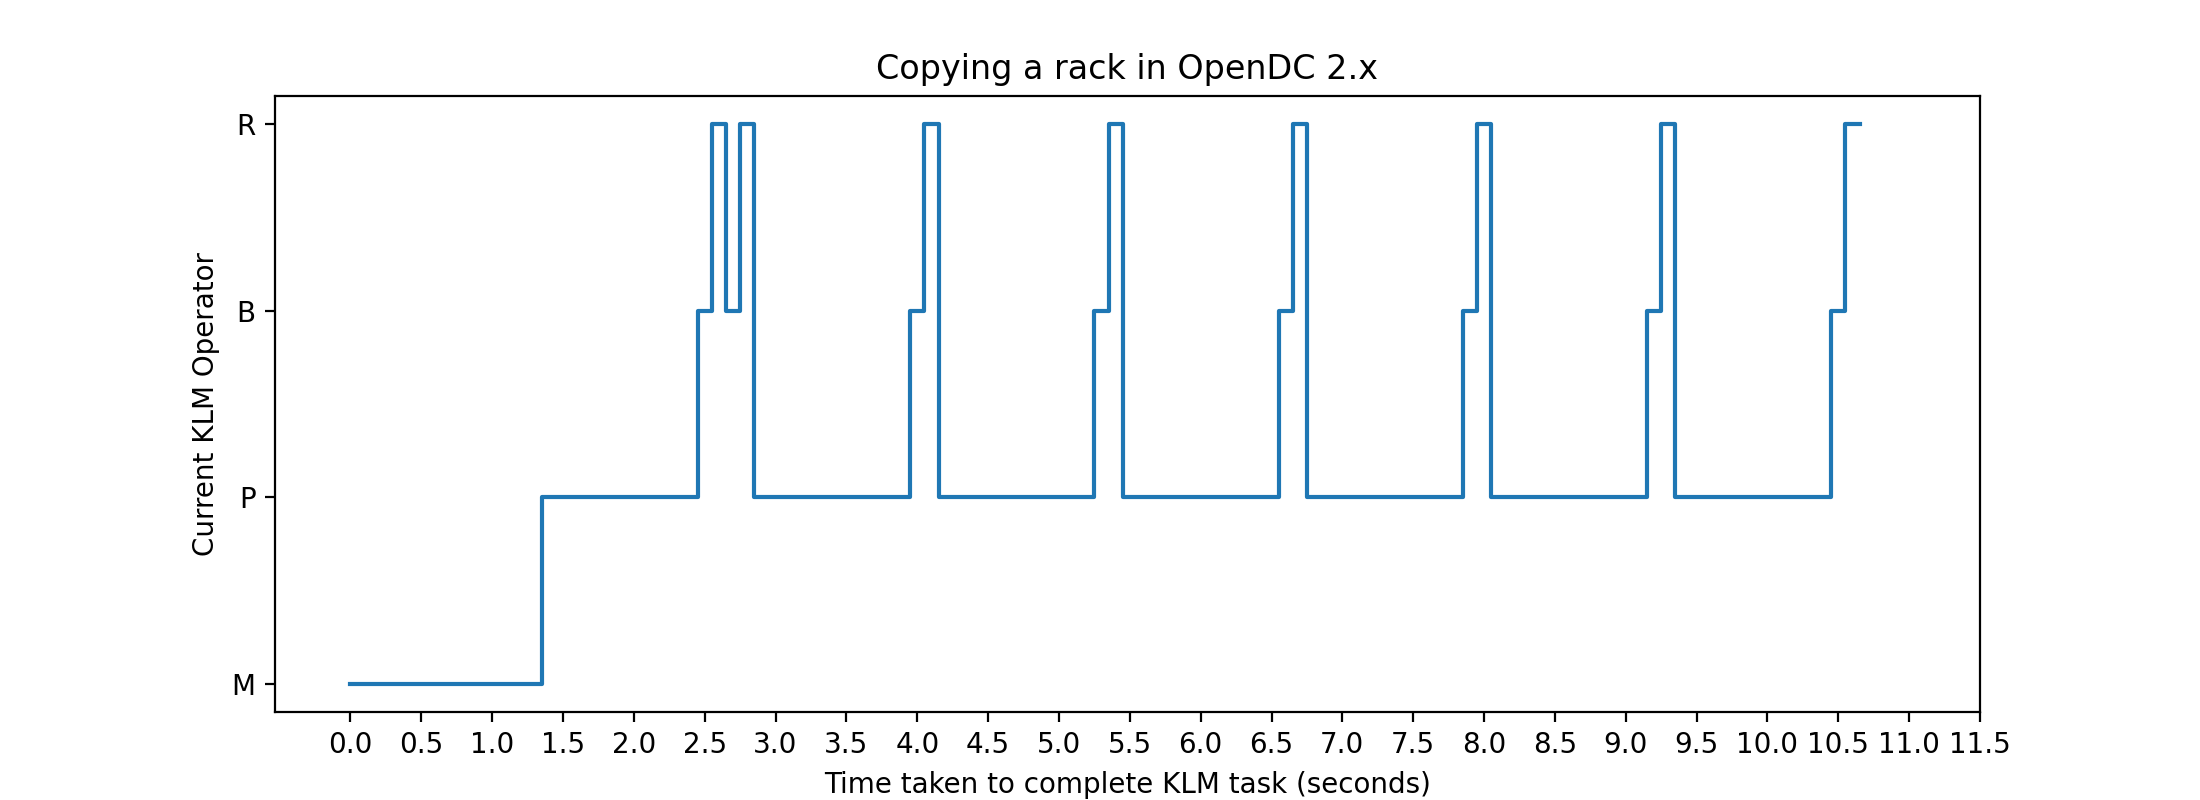
\includegraphics[width=\textwidth]{results/opendc2.png}
					\caption[Graph showing interactions required to complete a KLM task in \opendc{} with our extensions]{Graph showing interactions required to complete a KLM task in \opendc{} with prefabs.}
					\label{fig:opendcklm2}
				\end{subfigure}
				\label{fig:opendcklm}
			\end{figure}
			\begin{figure}[]
				\centering
				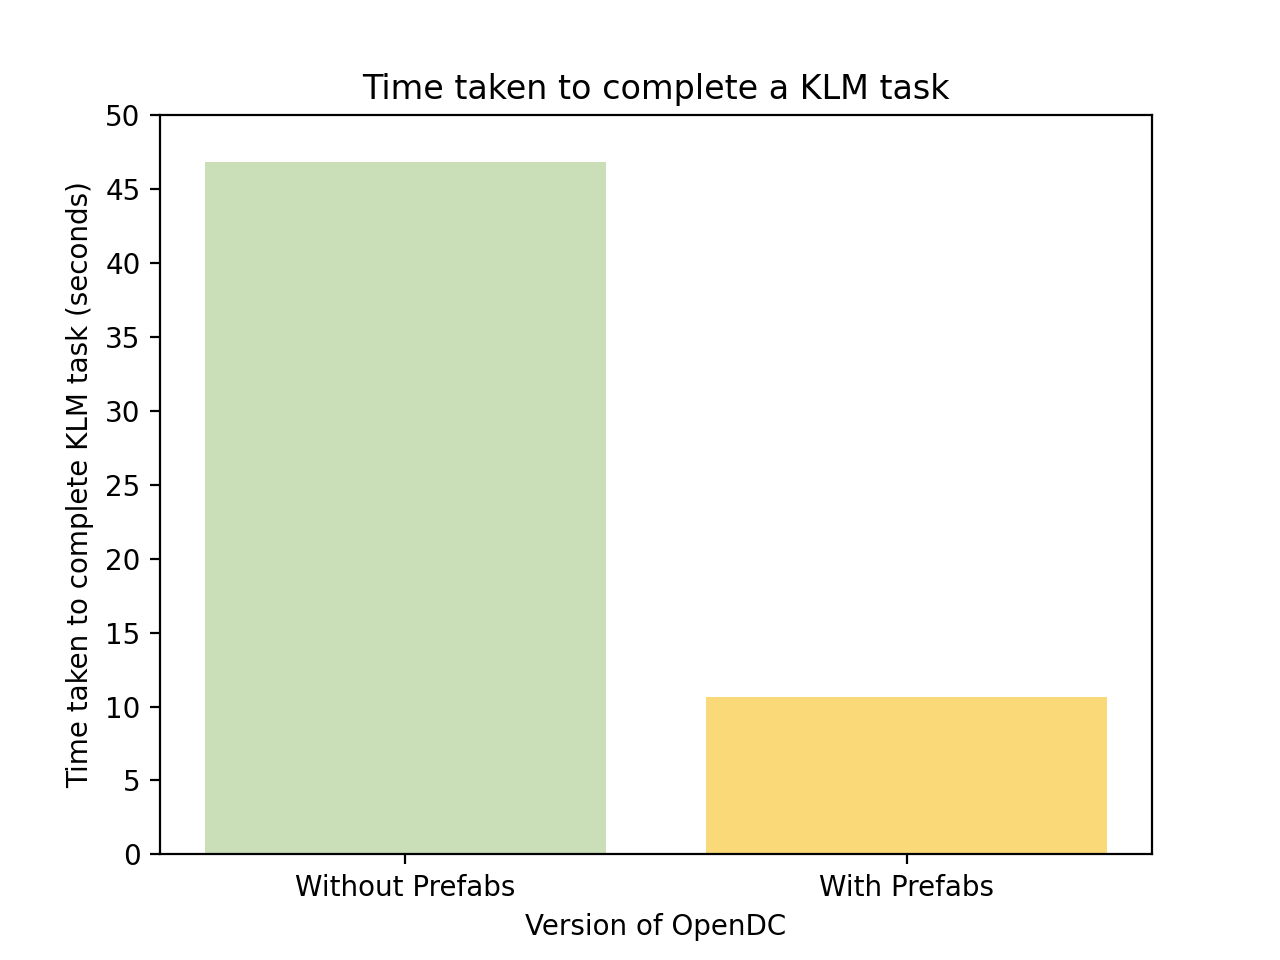
\includegraphics[width=0.5\textwidth]{results/klmbarcharts.png}
				\caption[Graph comparing time to complete a KLM task in two variants of \opendc{}]{Graph comparing time to complete a KLM task without and with prefabs.}
				\label{fig:opendcbarchart}
			\end{figure}

			From the results presented in Figures~\ref{fig:opendcklm1},~\ref{fig:opendcklm2} and~\ref{fig:opendcbarchart}, we can draw two conclusions.

			The first of these is that the number of interactions with the system is significantly reduced with the addition of prefabs.
			In Figure~\ref{fig:opendcklm1}, it can be seen that the process of copying the rack takes 70 discrete interactions.
			With less machines in the rack, version 1.x requires fewer interactions to perform the copy, but at the same time will take increasingly more time to copy as more machines are added.
			This is because each machine takes 18 interactions to copy after the initial rack has been created.
			At the same time, version 2.x requires just 15 interactions, regardless of the number of machines in the rack.
			It must also be noted that for our testing, we only use four components per machine.
			With more complex servers, the performance gaps grows even faster as machine are added.

			As a result of the reduced number of interactions required, we can also conclude that the time taken to copy a rack is reduced by the addition of prefabs.
			Using the values in Table~\ref{tab:3}, we can calculate the time required for version 1.x to complete a copy in our testing scenario using the below equation:
			$$M + 35P + 35B + 35R= 1.35 + 38.5 + 3.5 + 3.5= 46.85$$
			As a result, we can determine that it takes 46.85 seconds for an average user to complete the copy task defined in our testing setup without the use of prefabs.

			We then calculate the time taken for version 2.x to complete the task in the same way:
			$$M + 7P + 8B + 8R= 1.35 + 7.7 + 0.8 + 0.8= 10.65$$
			From these results, we can see that prefabs would allow an average user to complete the copy task in 10.65 seconds.
			This result suggests an almost 340\% speedup in the copy task as a result of prefabs.

			As a result, we consider our implementation of prefabs to show significant promise. We anticipate that a similar speedup will be possible in other aspects of \opendc{}, as more prefab operations are added to the \opendc{} codebase.

\newpage

\section{Conclusion} \label{sec:conclusion}
	In this section, we assess the suitability of our solution as a response to the problem presented in Section~\ref{sec:introduction}.
	We also discuss the future of this work, exploring ways in which this work could be further developed and improved, and how these ideas align with the vision for \opendc{} \cite{Iosup2017}.

	\subsection{Summary}
		Datacenter usage is growing fast, and will only continue to grow as more people use products that depend on cloud services.
		The growth of markets for IoT and game and content streaming will lead to even greater demand for datacenter capacity in the near future.
		As a result, it remains important that there are people equipped to design these new datacenters, and their expansions.
		With the extensions made to \opendc{} in this thesis, we intend to help broaden the field of people who are equipped to create these designs, allowing this explosive growth to continue.

		In this thesis, we have presented a design for a prefab data structure that is capable of expressing a wide variety of common datacenter hardware.
		Through creating a library of HPC prefabs, we have shown that this data structure is capable of accurately representing common datacenter hardware.
		Because of its use of JSON, the data structure is also easily extensible, supporting future work both in terms of the capabilities of \opendc{}, and in terms of server design.
		The JSON basis also provides a hierarchical organisational structure, in which components have a clear and logical place, allowing the structure itself to be easily readable and understandable.
		
		In addition to creating a design for prefabs, we have also successfully created a functional prototype for experimenting with the new technologies introduced with the prefabs extension.
		Our prototype, composed of a Python frontend, a Python command-line interface, and a MongoDB backend, supports many of the operations proposed in our design, and serves as a useful playground for testing additional features that could be added to prefabs.
		Creating prefabs in an environment based on the structure of \opendc{}, without fully implementing the design in \opendc{} allows for quick experimentation.
		This provides the ability to get rapid feedback while avoiding spending time implementing an idea into the broader \opendc{} codebase, making it easier to justify attempting a wider range of approaches to the problem.

		Lastly, in order to assess the use of prefabs in practice, we used KLM testing to show that operations on prefabs can provide a significant increase in prototyping speed.
		We find that KLM testing provides a simple to understand and easy to implement method of testing improvements made to ease of use, which we think will be of value in further extensions of \opendc{}.
		The improvements in performance found in our testing increase as the complexity of the datacenter increases, leading to even larger performance improvements for users tasked with designing massive-scale topologies.
		Now that the prefab data structure has been implemented in \opendc{}, along with an implementation of a desirable operation on prefabs, other operations can be easily added to the project to further increase usability and prototyping speed.
		We expect that, with user interface refinements, it may even be possible to further decrease the time taken to design a topology.
		In addition to validating the use of prefabs by using them to represent existing server hardware from a specific domain, we have proposed a method for doing so that is applicable to other domains.
		Using information provided by server OEMs to define our domain-specific prefabs is suitable for at least the larger domains within datacenter usage, if not also for smaller and emerging domains such as game streaming.
		However, we are limited in this approach to the domains that a given OEM chooses to target: smaller and emerging domains may not be considered large enough economically for an OEM to design for, leading to a reduced set of existing servers to model.
		However, we do find that our approach has been successful for the domain of HPC, producing high-quality representations of existing server SKUs currently offered on the market.


	\subsection{Future Work} \label{sec:future-work}
		Looking forward, there are several areas of interest that it would be beneficial to visit in future research.

		Firstly, there are many more characteristics of datacenter hardware that we could extend \opendc{} to represent. 
		We currently do not focus on high-density servers with multiple mainboards (such as blade servers) in each chassis in this thesis. 
		We could also extend rack prefabs to include networking hardware required for the topology. 
		The addition of networking hardware would also be beneficial for modelling \textit{Storage Area Networks} (SANs) and topologies that include nodes comprised of multiple units, such as HP's Superdome Flex concept\footnote{\url{http://hpe.com/superdome}}.
		Hardware for managing the power distribution throughout a topology would also be an important future expansion.
		Uninterruptible Power Supplies (UPSes) and Power Distribution Units (PDUs) are critical to the health of datacenter hardware, and take up rackspace.
		As a result, it would be useful to represent this hardware in \opendc{} in the future, as per-rack power limits would be dictated by the presence of such hardware.

		Next, the \opendc{} user interface could be further refined, to increase functionality and improve usability.
		A possible addition to the UI could be a powerful text-based console within the browser, so that the creation and manipulation of topologies and prefabs could become even more intuitive, allowing for even faster (and reproducible) prototyping.
		While the features we have introduced in this thesis are aimed towards a more general, less technically-oriented audience, the above feature would be aimed at users with more experience in datacenter design.

		Additionally, we could extend domain-specific prefabs to include more domains.
		So far, we have covered the domain of High Performance Computing, but there are many more that remain that are extremely relevant to the direction of the industry.
		Areas such as cloud gaming, or business-critical infrastructure have different requirements of their hardware choices, and so their topologies and thus their prefabs would likely look quite different from what we have explored so far in this thesis.
		Future work could investigate what kinds of hardware is used in these fields, and what useful prefabs would look like in these domains.

		Lastly, it would be interesting to design a means for \opendc{} to simulate user-specified workloads on systems designed by \opendc{} itself. 
		\opendc{} would be able to leverage a large database of performance data to make component choices based on the workload specified by the user. 
		\opendc{} could even be taught how to perform such a task, using Machine Learning with existing datacenter designs as training models.
		Research could be carried out to determine which hardware characteristics translate best into high performance for certain workloads, leading to objectively performant prefabs designed for those workloads.
		These research-based prefabs would then serve to validate the prefabs that \opendc{} learns to build, and further help develop this functionality.
		In this way, the system would be designed for the best objective performance at the specified workload, potentially adherent to specified constraints such as financial or power budget.
		If desired, the level of user interaction could be minimal to none, perhaps only requiring small changes to the design.







\newpage
% For more on bibliography styles, see 
% https://www.overleaf.com/learn/latex/Bibtex_bibliography_styles
\bibliographystyle{abbrv}
\bibliography{main}
\newpage
\appendix
\appendixpage
\addappheadtotoc
\begin{table}[]
			\centering
			\resizebox*{!}{\textheight}{%
				\begin{tabular}{lrlr}
					\toprule
					\multicolumn{2}{l}{version 1.x}                      & \multicolumn{2}{l}{version 2.x}                       \\ \midrule
					Move to target tile                      & 1.1       & Move mouse to target rack                       & 1.1 \\
					Click                                    & 0.1       & Click                                           & 0.1 \\
					Move to "start rack construction" button & 1.1       & Click                                           & 0.1 \\
					Click                                    & 0.1       & Move mouse to "save this rack to prefab" button & 1.1 \\
					Move back to target tile                 & 1.1       & Click "save this rack to prefab"                & 0.1 \\
					Click                                    & 0.1       & Move mouse to "back to room"                    & 1.1 \\
					Move to "stop rack construction" button  & 1.1       & Click "back to room"                            & 0.1 \\
					Click                                    & 0.1       & Move mouse to "load a rack from a prefab"       & 1.1 \\
					move to newly made rack                  & 1.1       & Click "load a rack from a prefab"               & 0.1 \\
					Click                                    & 0.1       & Move mouse to target prefab                     & 1.1 \\
					Move mouse to "add machine" button       & 1.1       & Click                                           & 0.1 \\
					Click                                    & 0.1       & Move mouse to "confirm import" button           & 1.1 \\
					Move mouse to "add machine" button       & 1.1       & Click                                           & 0.1 \\
					Click                                    & 0.1       & Move mouse to desired rack location             & 1.1 \\
					Move mouse to "add machine" button       & 1.1       & Click                                           & 0.1 \\
					Click                                    & 0.1       &                                                 &     \\
					Move mouse to machine one                & 1.1       &                                                 &     \\
					Click                                    & 0.1       &                                                 &     \\
					move mouse to "add" button               & 1.1       &                                                 &     \\
					Click                                    & 0.1       &                                                 &     \\
					Move mouse to "GPU" tab                  & 1.1       &                                                 &     \\
					Click                                    & 0.1       &                                                 &     \\
					move mouse to "add" button               & 1.1       &                                                 &     \\
					Click                                    & 0.1       &                                                 &     \\
					Move mouse to "memory" tab               & 1.1       &                                                 &     \\
					Click                                    & 0.1       &                                                 &     \\
					move mouse to "add" button               & 1.1       &                                                 &     \\
					Click                                    & 0.1       &                                                 &     \\
					Move mouse to "storage" tab              & 1.1       &                                                 &     \\
					Click                                    & 0.1       &                                                 &     \\
					move mouse to "add" button               & 1.1       &                                                 &     \\
					Click                                    & 0.1       &                                                 &     \\
					Move mouse to "back to rack" button      & 1.1       &                                                 &     \\
					Click                                    & 0.1       &                                                 &     \\
					Move mouse to machine two                & 1.1       &                                                 &     \\
					Click                                    & 0.1       &                                                 &     \\
					move mouse to "add" button               & 1.1       &                                                 &     \\
					Click                                    & 0.1       &                                                 &     \\
					Move mouse to "GPU" tab                  & 1.1       &                                                 &     \\
					Click                                    & 0.1       &                                                 &     \\
					move mouse to "add" button               & 1.1       &                                                 &     \\
					Click                                    & 0.1       &                                                 &     \\
					Move mouse to "Memory" tab               & 1.1       &                                                 &     \\
					Click                                    & 0.1       &                                                 &     \\
					move mouse to "add" button               & 1.1       &                                                 &     \\
					Click                                    & 0.1       &                                                 &     \\
					Move mouse to "Storage" tab              & 1.1       &                                                 &     \\
					Click                                    & 0.1       &                                                 &     \\
					move mouse to "add" button               & 1.1       &                                                 &     \\
					Click                                    & 0.1       &                                                 &     \\
					Move mouse to "back to rack" button      & 1.1       &                                                 &     \\
					Click                                    & 0.1       &                                                 &     \\
					Move mouse to machine three              & 1.1       &                                                 &     \\
					Click                                    & 0.1       &                                                 &     \\
					move mouse to "add" button               & 1.1       &                                                 &     \\
					Click                                    & 0.1       &                                                 &     \\
					Move mouse to "GPU" tab                  & 1.1       &                                                 &     \\
					Click                                    & 0.1       &                                                 &     \\
					move mouse to "add" button               & 1.1       &                                                 &     \\
					Click                                    & 0.1       &                                                 &     \\
					Move mouse to "memory" tab               & 1.1       &                                                 &     \\
					Click                                    & 0.1       &                                                 &     \\
					move mouse to "add" button               & 1.1       &                                                 &     \\
					Click                                    & 0.1       &                                                 &     \\
					Move mouse to "storage" tab              & 1.1       &                                                 &     \\
					Click                                    & 0.1       &                                                 &     \\
					move mouse to "add" button               & 1.1       &                                                 &     \\
					Click                                    & 0.1       &                                                 &     \\
					Move mouse to "back to rack" button      & 1.1       &                                                 &     \\
					Click                                    & 0.1       &                                                 &     \\ \midrule
					\textbf{M + 35P + 35B + 35R}             &           & \textbf{M + 7P + 8B + 8R}                       &     \\
					\textbf{= 1.35 + 38.5 + 3.5 + 3.5}       & \textbf{} & \textbf{= 1.35 + 7.7 + 0.8 + 0.8}               &     \\
					\textbf{= 46.85}                         & \textbf{} & \textbf{= 10.65}                                &     \\ \bottomrule
				\end{tabular}%
				}
				\caption{Results of KLM testing before and after the addition of prefabs.}
				\label{tab:results}
			\end{table}


\end{document}
% \end{document}

M + 7P + 8B + 8R= 1.35 + 7.7 + 0.8 + 0.8= 10.65
M + 35P + 35B + 35R= 1.35 + 38.5 + 3.5 + 3.5= 46.85
